\documentclass{article}
\usepackage[english]{babel}
\usepackage[utf8]{inputenc}
\usepackage{fancyhdr}
\usepackage{graphicx}
\usepackage{float}
\usepackage{listings}
\usepackage[parfill]{parskip}
\usepackage{fourier}

\pagestyle{fancy}
\fancyhf{}
\rhead{Proudly \LaTeX}
\lhead{Doing Survey Research 2018}
\rfoot{Page \thepage}
 
\begin{document}
 
\section*{\hfil Lab Worksheet II \hfil}
\subsection*{Stata's interface}

This is probably the first time you use Stata. As described in their own website, ``Stata is a complete, integrated statistics package that provides everything you need for data analysis, data management, and graphics.''
 
\begin{figure}[H]
	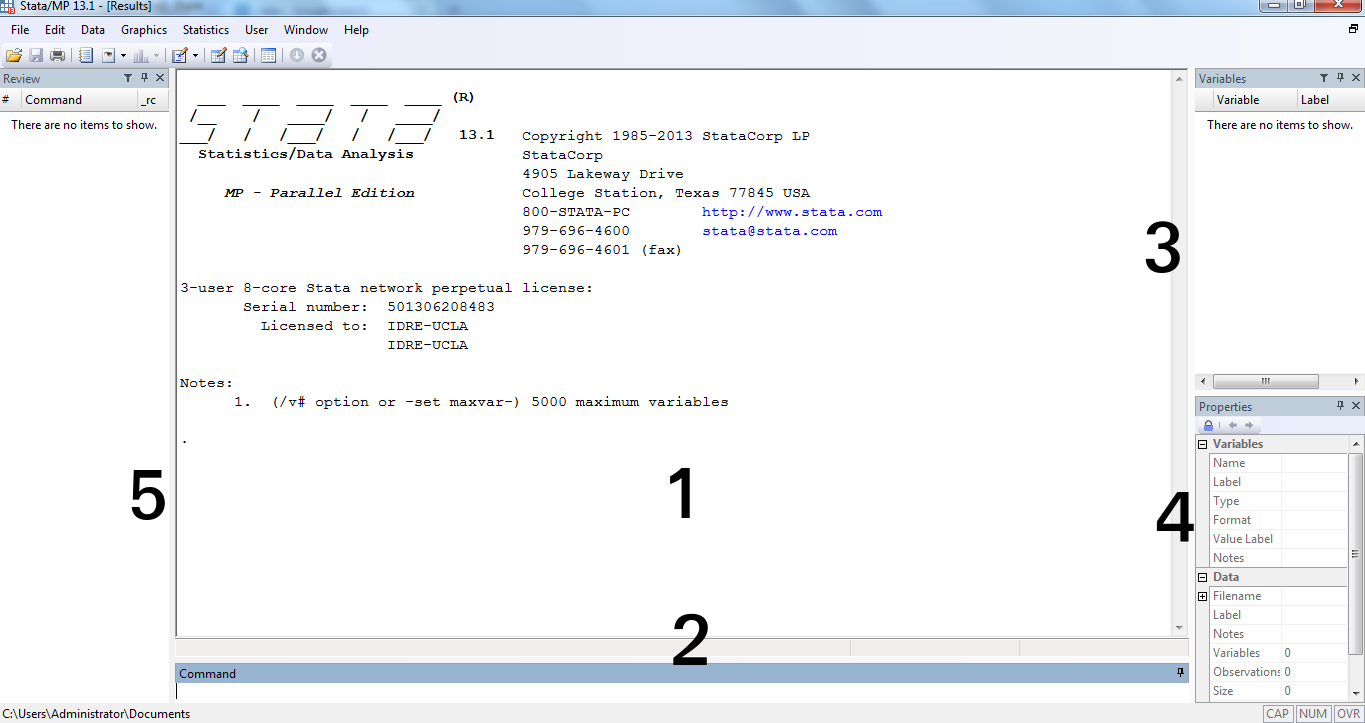
\includegraphics[width=\linewidth]{Stata_Interface.png}
	\caption{Stata's interface.}
\end{figure}

Upon starting Stata you will see the following sections:

\begin{enumerate}
	\item The results and outputs of your commands will be displayed in the \textbf{results window}.
	\item The \textbf{command window} is where you want to type your commands and send them to Stata by pressing the Enter key.
	\item If you have a dataset loaded its variables will appear in the \textbf{variables pane}.
	\item You can browse the properties of variables in the \textbf{properties pane}.
	\item The \textbf{review pane} lists all the actions you have taken in Stata.  
\end{enumerate}

At the moment you have no data loaded, that is the reason why your variables window is empty. Today you are going to input manually some data on UK universities. You can find these data in the table below.

\begin{table}[H]
	\begin{centering}
		\caption{Some universities in the UK}
	\end{centering}
\bigskip
	\begin{tabular}{r|c|c|c|c|c|c}
		\multicolumn{1}{c|}{\textbf{Name}}                                      & \textbf{Students} & \textbf{Ranking} & \textbf{Location}                                          & \textbf{\begin{tabular}[c]{@{}c@{}}Nobel\\ laureate\end{tabular}} & \textbf{\begin{tabular}[c]{@{}c@{}}Vice\\ chancellor\end{tabular}} & \textbf{Year} \\
		\begin{tabular}[c]{@{}r@{}}Edinburgh\\ University\end{tabular}         & 35258             & 20               & Scotland                                                   & 20                                                                & Male                                                               & 1582          \\ \hline
		\begin{tabular}[c]{@{}r@{}}Napier\\ University\end{tabular}            & 17264             & 64               & Scotland                                                   & 0                                                                 & Female                                                             & 1992          \\ \hline
		\begin{tabular}[c]{@{}r@{}}University\\ of Essex\end{tabular}          & 11939             & 47               & England                                                    & 2                                                                 & Male                                                               & 1965          \\ \hline
		\begin{tabular}[c]{@{}r@{}}University of\\ Cambridge\end{tabular}      & 18271             & 1                & England                                                    & 91                                                                & Male                                                               & 1209          \\ \hline
		\begin{tabular}[c]{@{}r@{}}Cardiff\\ University\end{tabular}           & 30180             & 27               & Wales                                                      & 2                                                                 & Male                                                               & 1997          \\ \hline
		\begin{tabular}[c]{@{}r@{}}University of\\ Liverpool\end{tabular}      & 21276             & 59               & England                                                    & 9                                                                 & Female                                                             & 1903          \\ \hline
		\begin{tabular}[c]{@{}r@{}}Queen's\\ University\\ Belfast\end{tabular} & 24955             & 45               & \begin{tabular}[c]{@{}c@{}}Northern\\ Ireland\end{tabular} & 3                                                                 & Male                                                               & 1908          \\ \hline
		\begin{tabular}[c]{@{}r@{}}Glasgow\\ Caledonian\end{tabular}           & 18410             & 89               & Scotland                                                   & 1                                                                 & Female                                                             & 1993          \\ \hline
		\begin{tabular}[c]{@{}r@{}}Ulster\\ University\end{tabular}            & 26200             & 82               & \begin{tabular}[c]{@{}c@{}}Northern\\ Ireland\end{tabular} & 0                                                                 & Male                                                               & 1982          \\ \hline
		\begin{tabular}[c]{@{}r@{}}University of\\ Warwick\end{tabular}        & 23420             & 6                & England                                                    & 1                                                                 & Male                                                               & 1965         
	\end{tabular}
\end{table}

As you can see there are seven variables and ten observations. You need the following variables:

\begin{itemize}
	\item Name of university.
	\item Total number of students (numeric).
	\item Position in the The Guardian Ranking.
	\item Geographical location (categorical, see below).
	\item Number of affiliated Nobel laureates (numeric).
	\item Gender of the Vice-chancellor (binary, see below).
	\item Year in which it was established (numeric).
\end{itemize}

The variable ``Location'' has the following four categories: Scotland = 1, Northern Ireland = 2, Wales = 3, and England = 4. The variable ``Vice-chancellor'' should be coded as Male = 0 and Female = 1.

You need to think of suitable \textbf{variable names}, \textbf{variable labels}, and \textbf{value labels}. Keep in mind that is customary, but not mandatory, to name variables with small letters. Stata accepts both upper cases and lower cases, but it is case sensitive! Also, variable names cannot contain spaces and the use of underscores is customary when signalising spaces. After thinking of some variable names, open up the data editor by clicking on the icon with a pencil over a spreadsheet (see Figure 2). Stata's data editor resembles very much Excel. Your ``spreadsheet'' should be empty, but if it was not you could type \texttt{clear all} in the command window to get rid of previous data.

\begin{figure}[H]
	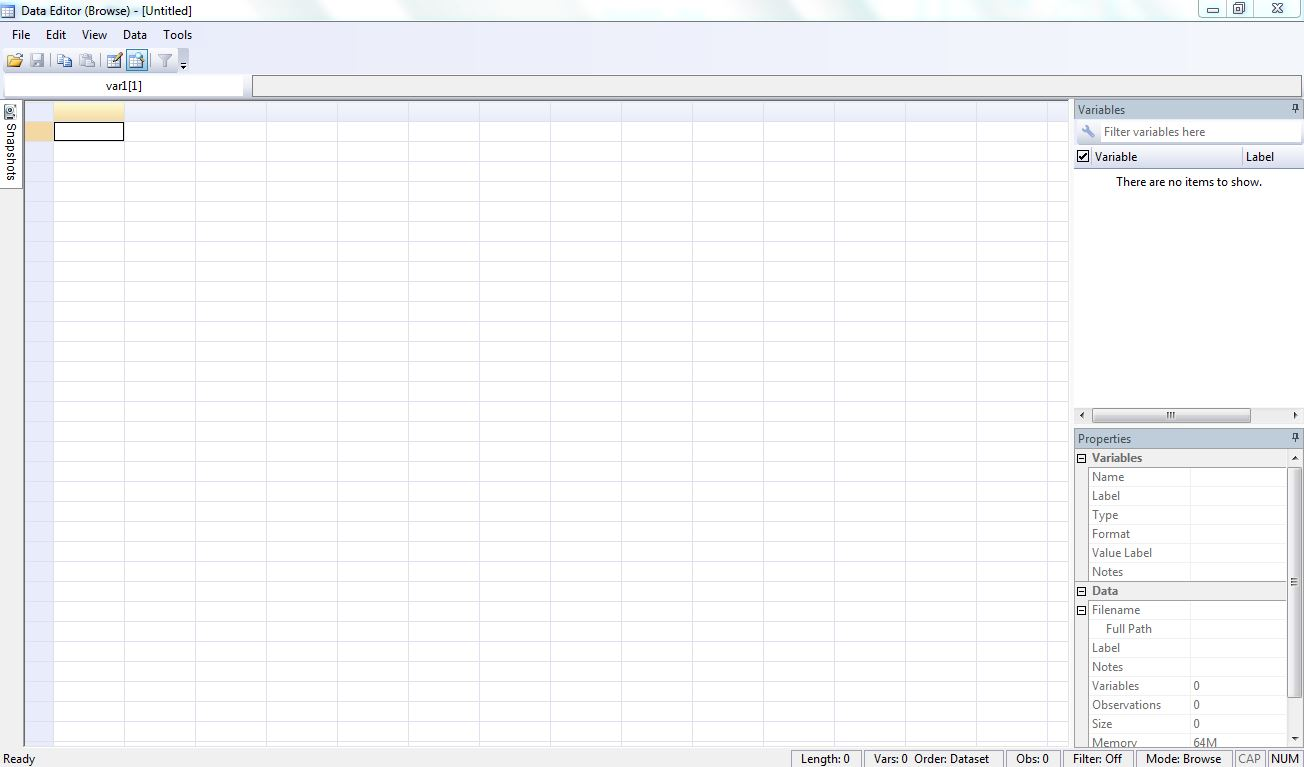
\includegraphics[width=\linewidth]{Stata_Data_Editor_Blank.JPG}
	\caption{Stata's data editor.}
\end{figure}

Now it is time to enter the data; start by typing in the first observation (University of Edinburgh). If you press the Tab key you will move onto the next cell. Keep entering the values for all variables for the University of Edinburgh (your first observation). Here it is important to remember that rows represent observations whereas columns represent variables. You might notice that Stata is naming your variables as \textit{var1}, \textit{var2}, and so on. To change \textbf{variable names} simply select a variable in the variables pane (top right corner) and change its name in the properties pane (bottom right corner). Repeat the process for the rest of variables. Let me remind you again that we need a number for geographical location and gender (the categories are specified above).

From the properties pane you can also define \textbf{variable labels}. The process is identical as before: select a variable in the variables pane, switch to the properties pane and give the variable a label (but this time using the box named ``Label''). Variable labels allow spaces. Remember to be precise and accurate with your labelling, but try to keep your labels parsimonious (not too short as to make them ambiguous, but not too long either). Once you have named and labelled your variables you should see the new names and labels in the variables window.

Now that you have assigned names and labels to all your variables, you are going to assign \textbf{value labels} to two variables: geographical location and vice-chancellor (remember the above-mentioned specifications). But first try typing in the command window:

\begin{lstlisting}
	tabulate gender
\end{lstlisting} 

In the command above, \texttt{tabulate} creates a tabulation of a variable named ``gender.'' If you did not name your variable ``gender'', you will have to substitute in your variable's name instead of ``gender.'' In the results window you can see now a table with two categories: 0 and 1. You know that 0 = Male and 1 = Female, but when you report these results you want your readers to know exactly what is going on. Changing 0 to ``Male'' and 1 to ``Female'' is what you do when you assign \textbf{value labels} to your vice-chancellor's gender variable.

\begin{figure}[H]
	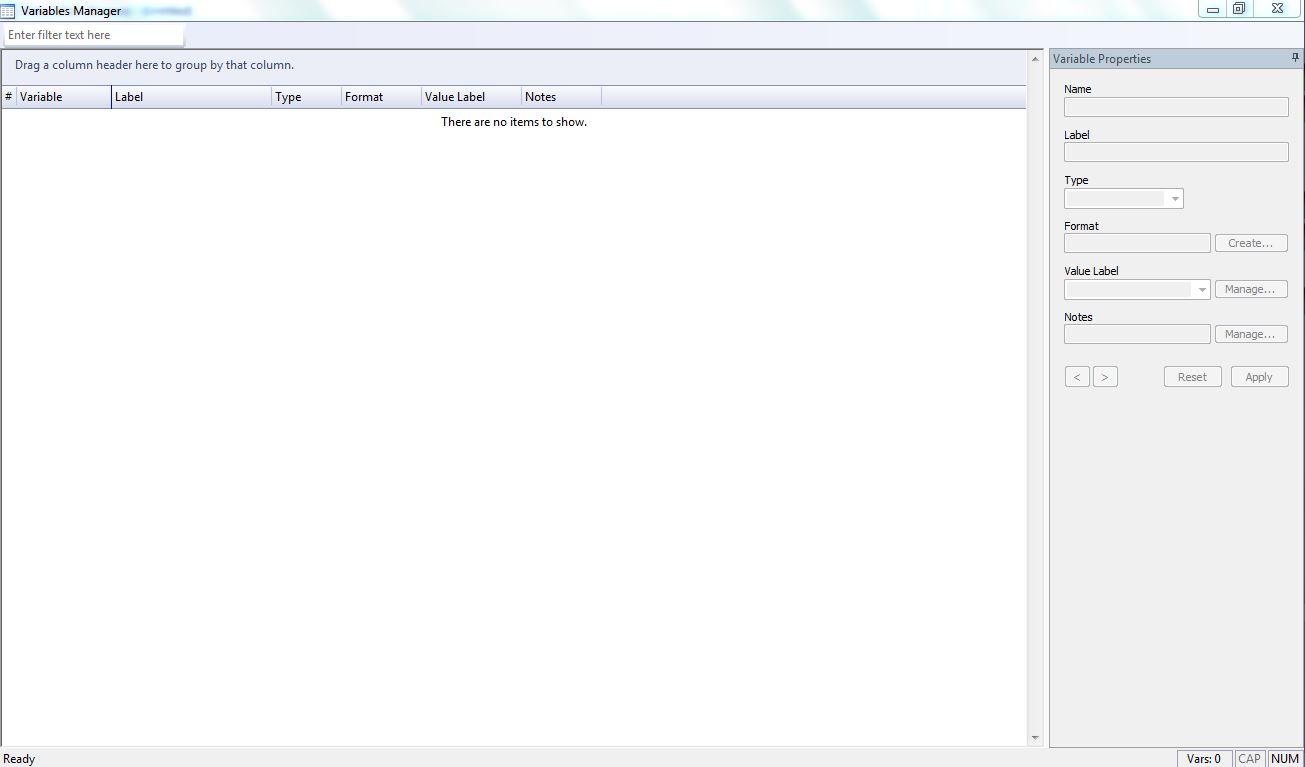
\includegraphics[width=\linewidth]{Stata_Variables_Manager.JPG}
	\caption{Stata's variables manager.}
\end{figure}

To assign value labels you need to exit the data editor and open the \textit{variables manager}. This can be accessed by clicking on the icon with a spreadsheet. Once the variables manager shows up (see Figure 3 for the generic, blank window) you need to create first a set of value labels which you will be attaching to a specific variable later on. Click on \textbf{Manage...} (situated on the right side of the window). In the new window click on \textbf{Create Label}. Yet a new window named \textbf{Create Label} will appear on screen. Give to your new set of value labels a name (in the \textbf{Label name} box). It is best if you name it with something that resembles the name of the variable you are modifying. For example, if you created a variable named ``location'' for the geographical location of universities you can name your set of value labels as ``locationlab'' or ``locationl.'' Keep in mind that sets of value labels cannot use variable names. Now type in the box named \textbf{Value} the original value you gave to your variable (i.e., 0 = Male, so you would type ``0'' here) and in the \textbf{Label} box type its new label (i.e., ``Male''). Then click on \textbf{Add} and repeat the process for 1 = Female. Once this is done click on \textbf{OK}.

Now that you have a set of value labels, the last thing you need to do is attach that set to the original variable. For this, go back to the variables manager window (Figure 3), select the variable at stake, and click on the down arrow located to the right of \textbf{Value Label}. A dropdown menu in which you can select the appropriate set of value labels will appear. Finally, click on \textbf{Apply}. If you use the \texttt{tabulate} command again you will see that your tabulation, this time, reports ``Female'' and ``Male'' instead of 1 and 0. Well done!

\end{document}